% !TEX encoding = UTF-8
% !TEX program = pdflatex
% !TEX root = InformationRetrieval.tex
% !TEX spellcheck = it-IT

\section{Esame 2015-02-04}

\subsection{Domanda 1}

Si illustri lo schema a ``U''

\subsubsection{Soluzione}

Lo schema a ``U'' non è altro che una visione ad alto livello di un sistema IR.

\begin{figure}[htbp]
	\centering
	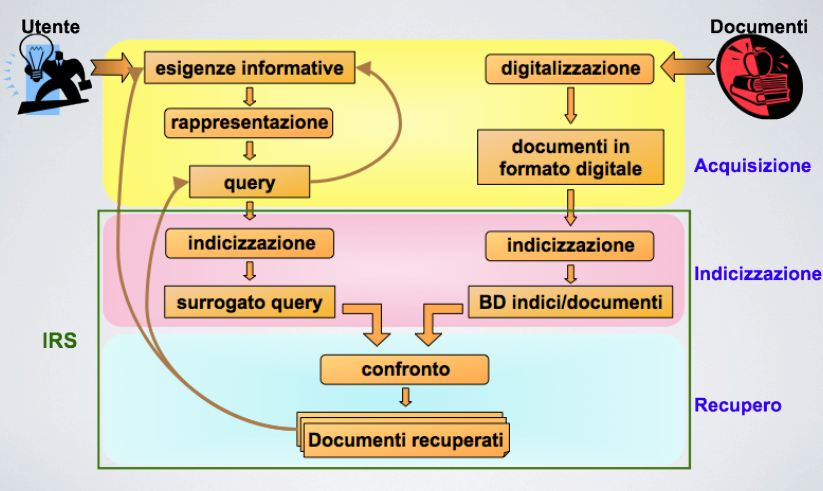
\includegraphics[width=.8\textwidth]{images/es-3-fig-1.png}
\end{figure}

Da una parte della ``U'' c'è il ramo relativo all'esigenza informativa dell'utente, la quale viene rappresentata da una query. Dall'altra parte c'è la collezione dei documenti, che contiene tutti i dati che devono essere indicizzati dal sistema in modo che possa fornire delle risposte all'utente.

Ad entrambi i rami viene poi applicato lo stesso processo di indicizzazione. Viene così ottenuta un'indice dei documenti che rappresenta in modo più semplice le informazioni contenute nei vari documenti. La stessa trasformazione subita dai documenti viene applicata in parallelo anche alla query effettuata dall'utente. 

In questo modo quando i due rami della ``U'' si congiungono nel modello di reperimento, questi possono essere facilmente confrontati tra loro. Ad esempio sia la query che i documenti della collezione possono essere rappresentati da un vettore binario che specifica se determinati termini compaiono all'interno della query/documento.

Una volta confrontata la query il sistema di reperimento produce come risultato o il documento più simile alla query, oppure una lista di documenti ordinata per similarità.

\subsection{Domanda 2}

Si effettui l'indicizzazione automatica dei documenti...

\subsection{Domanda 3}

Nel BIM la probabilità che un documento sia rilevante $P(\rel |D)$ è proporzionale al logaritmo del rapporto delle probabilità $P(\rel | D)$ e $P(\notrel | D)$. In cui $D$ è un vettore di variabili binarie.

A partire dal rapporto ottenere la formula del relevance weight:

$$
RW_i = \log \bigg( \frac{N_{t_iR} + 0.5}{N_R - N_{t_iR} +0.5} \frac{N_{NR} - N_{t_iNR} + 0.5}{N_{t_iNR} +0.5} \bigg)
$$

Utilizzando $p_i = \frac{N_{t_iR} +0.5}{N_R + 1}$.

\noindent Supponendo poi di avere la matrice 

\begin{table}[htbp]
	\centering
	\begin{tabular}{c|c|c|}
		\cline{2-3}
		& $t_1$ & $t_2$ \\ \hline
		\multicolumn{1}{|c|}{$d_1$} & 1  & 0  \\ \hline
		\multicolumn{1}{|c|}{$d_2$} & 0  & 5  \\ \hline
		\multicolumn{1}{|c|}{$d_3$} & 4  & 0  \\ \hline
		\multicolumn{1}{|c|}{$d_4$} & 0  & 3  \\ \hline
	\end{tabular}
\end{table}

\noindent calcolare i pesi per i due termini in assenza di informazioni sulla rilevanza dei documenti e senza usare la calcolatrice.

\subsubsection{Soluzione}

\begin{align}
P(\rel |D) &\propto \log \bigg( \frac{P(\rel | D)}{P(\notrel | D)} \bigg) \\
&= \log \bigg(  \frac{P(D | \rel)P(\rel)}{P(D)}  \frac{P(D)}{P(D | \notrel)P(\notrel)} \bigg) \quad \text{per Bayes}\\
&= \log \bigg(  \frac{P(D | \rel)}{P(D | \notrel)}  \underbrace{\frac{P(\rel)}{P(\notrel)}}_{\text{costante per tutta la collezione collezione}}\bigg)\\
&= \log \bigg(  \frac{P(D | \rel)}{P(D | \notrel)} \bigg)\\
&= \log \bigg(  \frac{\prod\limits_{i=1}^{|V|} P(t_i | \rel)}{\prod\limits_{i=1}^{|V|} P(t_i | \notrel)} \bigg) \quad \text{Naive bayes assumption} \\
&= \log \bigg(  \frac{\prod\limits_{i=1}^{|V|} p_i^{t_i}(1-p_i)^{1-t_i}}{\prod\limits_{i=1}^{|V|}q_i^{t_i}(1-q_i)^{1-q_i}} \bigg) \quad \text{variabili aleatori bernoulliane}\\
&= \log \bigg( \prod\limits_{i=1}^{|V|} \frac{ p_i^{t_i}(1-p_i)^{1-t_i}}{q_i^{t_i}(1-q_i)^{1-t_i}} \bigg)  \\
&= \sum\limits_{i=1}^{|V|} \log \bigg(  \frac{ p_i^{t_i}(1-p_i)^{1-t_i}}{q_i^{t_i}(1-q_i)^{1-t_i}} \bigg)\\
&= \sum\limits_{i=1}^{|V|} \log \bigg(  \frac{ \frac{p_i^{t_i}}{(1-p_i)^{t_i}}(1-p_i)  }{ \frac{q_i^{t_i}}{(1-q_i)^{t_i}}(1-q_i)  } \bigg)\\
&= \sum\limits_{i=1}^{|V|} \log \bigg(  \frac{ \bigg(\frac{p_i}{1-p_i} \bigg)^{t_i}  (1-p_i) }{ \bigg(\frac{q_i}{1-q_i}\bigg)^{t_i} (1-q_i)  } \bigg)\\
&= \sum\limits_{i=1}^{|V|} \log \bigg(   \bigg(\frac{p_i(1-q_i)}{(1-p_i)q_i} \bigg)^{t_i}  \underbrace{\frac{(1-p_i)}{(1-q_i) }}_{\text{costante per tutta la collezione}} \bigg)\\
&\propto \sum\limits_{i=1}^{|V|} t_i \log \bigg( \frac{p_i(1-q_i)}{(1-p_i)q_i} \bigg)
\end{align}

Per ottenere $RW_i$ è sufficiente espandere $p_i$ e $q_i$.

Per il secondo punto, non avendo a disposizione informazioni sui documenti rilevanti si ha che:

\begin{itemize}
\item $RW_1 = \log \bigg( \cfrac{0 + 0.5}{0 - 0 +0.5} \cfrac{4 - 2 + 0.5}{2 +0.5} \bigg) = \log\bigg(\cfrac{2.5}{2.5}\bigg) = \log(1) = 0$
\item $RW_2 = \log \bigg( \cfrac{0 + 0.5}{0 - 0 +0.5} \cfrac{4 - 2 + 0.5}{2 +0.5} \bigg) = \log\bigg(\cfrac{2.5}{2.5}\bigg) = \log(1) = 0$
\end{itemize}

\subsection{Domanda 4}

Dato un pool e una run, determinare:

\begin{enumerate}
	\item Il valore di precisione e richiamo con cut-off a 10, considerando come rilevanti tutti i documenti con grado superiore a \texttt{NR}.
	\item Il DCG della run con cut-off a 5, 10, 20 calcolato con base 10 e schema di pesatura \texttt{NR = 0, PR=5, FR=10, HR=15}
	\item Il DCG della run ideale a cut-off 15 e base 10.
\end{enumerate}

\subsubsection{Soluzione}

\begin{enumerate}
	\item $prec@10 = \cfrac{1 + 1 + 1 + 0 + 0 + 1 + 0 + 0 + 1 + 1}{10} = \cfrac{6}{10}$ e $recall@k = \cfrac{6}{12}$
	
	\item
	$$
	DCG@j = \sum\limits_{k = 1}^{j} dg_{r_t}^b[k]
	$$
	
	$$
	dg_{r_t}^b[k] = \begin{cases}
	r_t[k] & k < b \\
	\cfrac{r_t[k]}{\log_b k}
	\end{cases}
	$$
	\begin{itemize}
		\item $DCG@5 = 15 + 15 + 5 + 0 + 0 = 35$
		\item $DCG@10 = 15 + 15 + 5 + 0 + 0 + 10 + 0+ 0 + 15 + 10 = 70$
		\item $DCG@20 = DGC@10 + \cfrac{10}{\log_{10}11} + \cfrac{5}{\log_{10}12} + \ldots $
	\end{itemize}

	\item $IDCG@15 = 15 \times 4 + 10 \times 3 + 5 \times 3 + \cfrac{5}{\log_{10}11} + \cfrac{5}{\log_{10}12} + \cfrac{5}{\log_{10}13} +\cfrac{0}{\log_{10}14} +\cfrac{0}{\log_{10}15} $
\end{enumerate}

\subsection{Domanda 5}

Si presentino quali sono le differenze architetturali più significative fra un sistema di biblioteca digitale e un sistema di reperimento dell'informazione

\subsubsection{Soluzione}

Un sistema per una biblioteca digitale può essere implementato sia con un DBMS che come sistema IR.
Nel caso di un implementazione con un DBMS le interrogazioni che possono fare gli utenti sono più strutturate, ad esempio "tutti i libri scritti da" o "tutti i libri che hanno la categoria X" e i risultati forniti corrispondo ad un match deterministico della query dell'utente.

Lo stesso sistema può essere implementato anche come un IRS, in questo caso la query può anche essere più complessa, in formato narrativo e più ampia, ad esempio può essere la descrizione testuale dell'argomento trattato del libro.
Sarà poi l'IRS sottostante che si occuperà di indicizzare la query allo stesso modo dei documenti della collezione per calcolare la similarità con i documenti.

Da notare che con la versione DBMS questo tipo di interrogazione non può essere fatto, perché tipicamente nel database non viene memorizzato tutto il testo dei libri, mentre in un IRS viene utilizzato l'indice trasposto, che contiene maggiori informazioni riguardo il contenuto dei libri.

Un IRS inoltre può supportare lo stesso tipo di query di un DBMS, andando o a integrarlo, oppure ad estendere l'indice trasposto, aggiungendo dei termini extra, che non compaiono dei documenti, e che contengono l'informazione relativa agli autori e/o alla categoria del libro. Ovvero si può aggiungere all'indice un termine ``Mario Rossi'' e aggiungere alla posting-list del termini i pointer e tutti i documenti scritti da Mario Rossi.













